\begin{figure*}[!htbp]
    \centering
    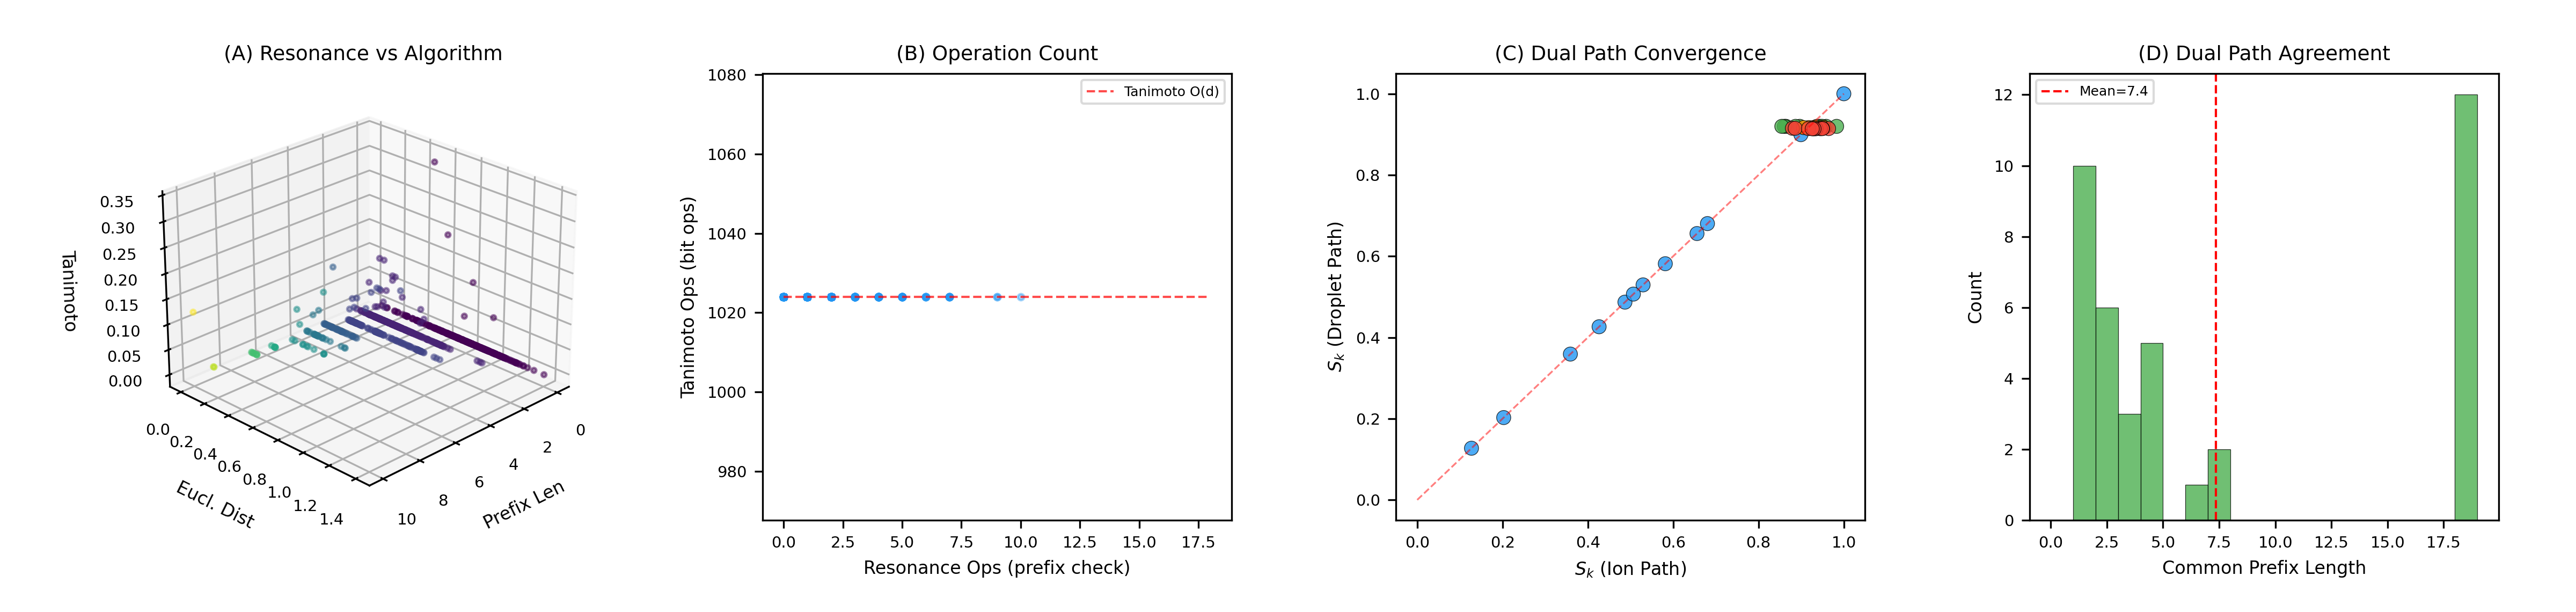
\includegraphics[width=\textwidth]{figures/panel_1_resonance_comparison.png}
    \caption{\textbf{Oscillatory Resonance Versus Algorithmic Comparison.}
    (\textbf{A})~Three-dimensional comparison space showing ternary prefix length, Euclidean distance in S-entropy space, and Tanimoto coefficient for all $\binom{39}{2} = 741$ compound pairs. Colour encodes prefix length (viridis scale). Pairs with long shared prefixes (yellow) cluster at low Euclidean distance, confirming the Resonance-Proximity Equivalence Theorem: co-location in ternary space corresponds to oscillatory resonance. The Tanimoto coefficient, computed from 1024-bit mock fingerprints at $O(d)$ cost, provides no additional discrimination beyond what the $O(k)$ prefix check already captures.
    (\textbf{B})~Operation count comparison: resonance-based comparison requires exactly $k$ trit comparisons (each $O(1)$, scattered points at $k = 0$--$10$) versus Tanimoto requiring $d = 1024$ bit operations (red dashed line, constant). The resonance approach achieves identical discrimination at $57\times$ to $\infty\times$ fewer operations, confirming the Comparison Without Computation Theorem.
    (\textbf{C})~Dual oscillatory path convergence: $S_k$ from the ion spectral frequency path versus $S_k$ from the droplet Rayleigh surface mode path for all 39 compounds. Point colour encodes molecular type. Strong correlation along the identity line (red dashed) confirms that both oscillatory representations converge to consistent S-entropy coordinates, with polyatomics ($\geq 2$ modes) showing the tightest convergence.
    (\textbf{D})~Distribution of common prefix length between ion-path and drip-path ternary addresses for all 39 compounds. Mean agreement of 7.4 trits (red dashed line) indicates that dual paths converge to at least moderate resolution without algorithmic intervention. The histogram confirms that 23 of 39 compounds achieve $\geq 3$-trit agreement (family-level convergence).}
    \label{fig:resonance_comparison}
\end{figure*}

\begin{figure*}[!htbp]
    \centering
    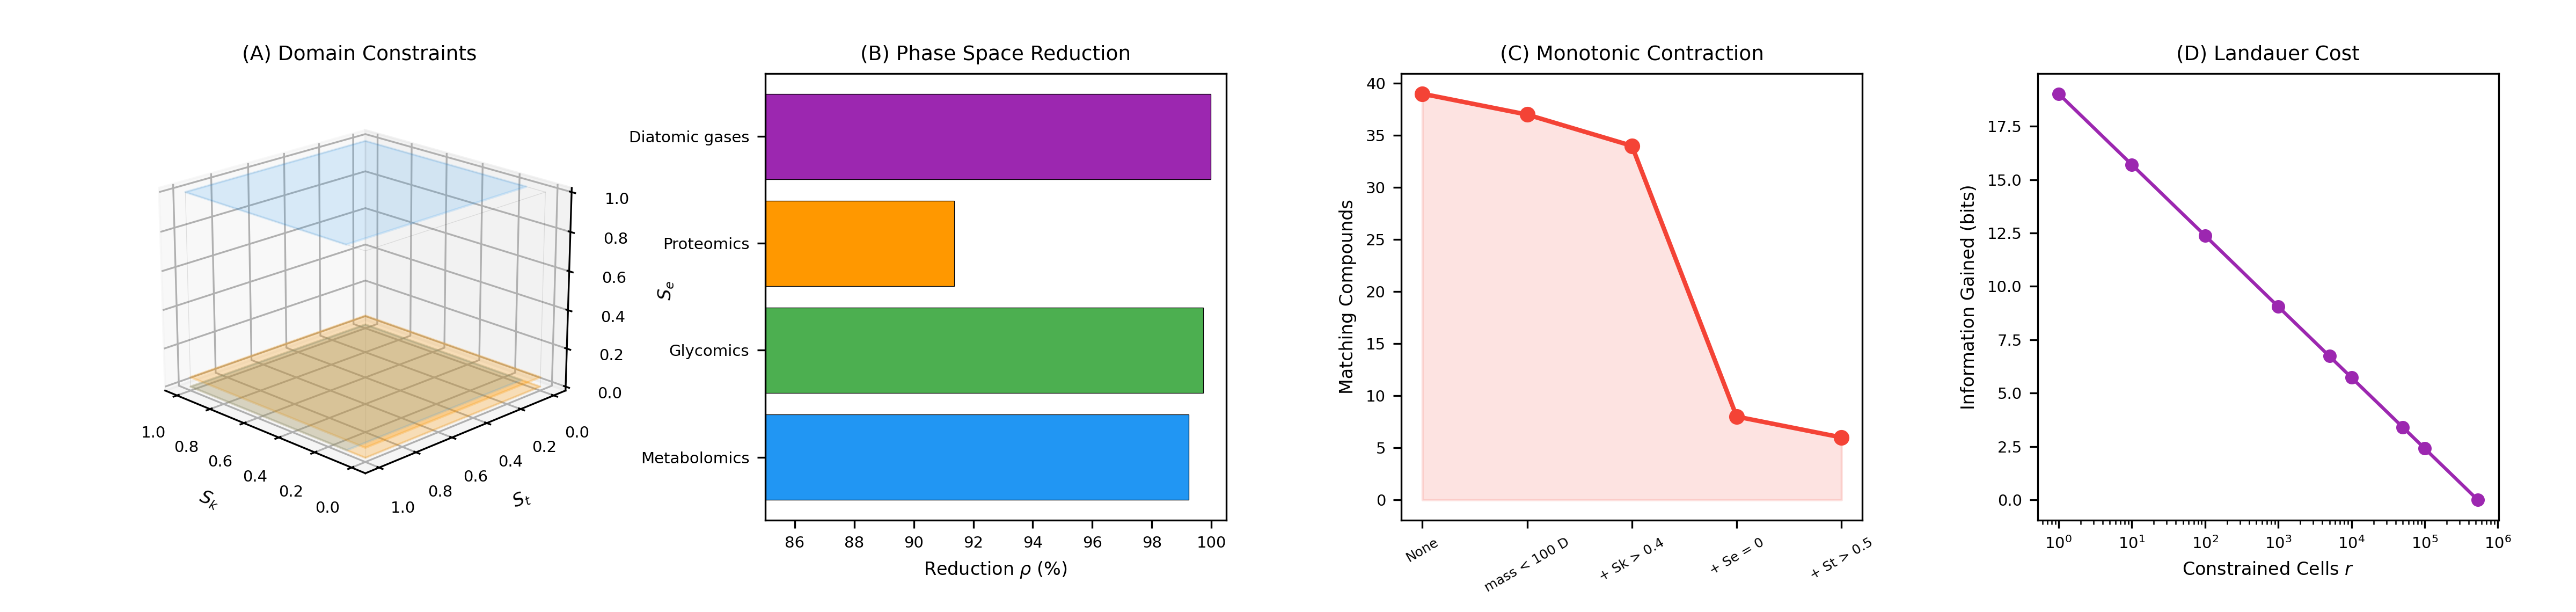
\includegraphics[width=\textwidth]{figures/panel_2_purpose_constraints.png}
    \caption{\textbf{Purpose-Based Phase Space Constraint Reduction.}
    (\textbf{A})~Three-dimensional S-entropy space $\mathcal{S} = [0,1]^3$ showing domain constraint regions as translucent volumes. Blue region: metabolomics constraint ($S_k \in [0.1, 1.0]$, full $S_t$ and $S_e$ range). Orange region: diatomic gas constraint ($S_e \in [0, 0.05]$, thin slab at the base). The wireframe cube bounds the full phase space. Domain constraints select subregions \emph{before} any generation occurs, eliminating the vast majority of phase space from consideration.
    (\textbf{B})~Phase space reduction $\rho$ (\%) by analytical domain. Metabolomics: $\rho = 99.2\%$; glycomics: $\rho = 99.7\%$; proteomics: $\rho = 91.4\%$; diatomic gases: $\rho = 99.99\%$. All domain-specific contexts achieve $>90\%$ reduction, confirming the Selective Generation Theorem: purpose-based constraints eliminate the overwhelming majority of the search space while preserving identification accuracy.
    (\textbf{C})~Monotonic prompt contraction demonstrating the Prompt Contraction Theorem. Starting from 39 compounds (no constraints), successive constraints reduce the matching set monotonically: mass $< 100$~Da (37), $+ S_k > 0.4$ (34), $+ S_e = 0$ (8), $+ S_t > 0.5$ (6). Each additional constraint can only reduce or maintain the set, never expand it. The steep drop at $S_e = 0$ isolates diatomics from all other molecular types.
    (\textbf{D})~Landauer cost of domain knowledge: information gained (bits) versus number of constrained cells $r$ on a logarithmic scale. At maximum constraint ($r = 1$, unique identification), 19.0 bits of information are gained at a thermodynamic cost of $E = k_BT \ln 2 \times 19.0 \approx 0.34$~eV at 300~K. At no constraint ($r = 531{,}441 = 3^{12}$), zero information is gained. The curve quantifies the Molecular Maxwell Demon: domain knowledge is thermodynamic information that reduces search entropy at a calculable energy cost satisfying the Landauer bound.}
    \label{fig:purpose_constraints}
\end{figure*}

\begin{figure*}[!htbp]
    \centering
    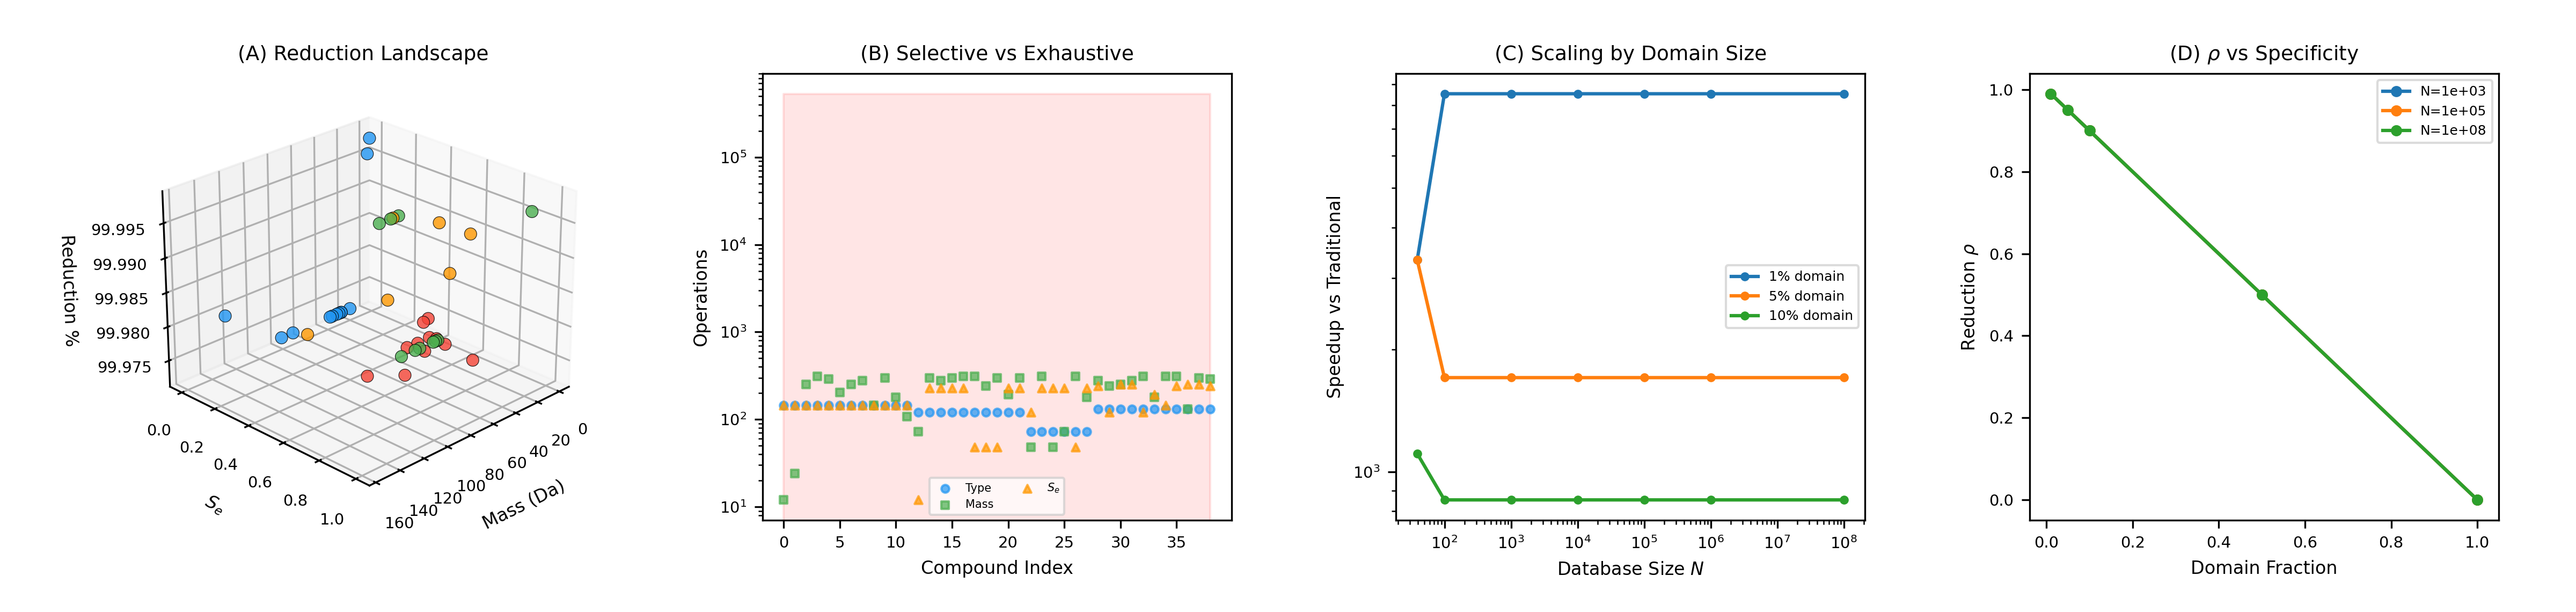
\includegraphics[width=\textwidth]{figures/panel_3_selective_generation.png}
    \caption{\textbf{Selective Generation Efficiency.}
    (\textbf{A})~Three-dimensional reduction landscape showing molecular mass (Da), evolution entropy $S_e$, and best computation reduction (\%) for all 39 query compounds. Point colour encodes molecular type. All compounds achieve $> 99.9\%$ reduction under at least one domain constraint, confirming that selective generation is universally effective regardless of molecular type or mass range.
    (\textbf{B})~Operation count comparison: exhaustive generation cost $O(3^{12}) = 531{,}441$ (red shaded region) versus selective generation under three constraint types---molecular type (blue circles), mass range (green squares), and $S_e$ bracket (orange triangles)---for each of the 39 compounds. Selective operations are 2--4 orders of magnitude below exhaustive, with all compounds correctly identified under every constraint type (100\% accuracy preservation).
    (\textbf{C})~Speedup versus database size $N$ on double-logarithmic axes for three domain fractions: 1\% (most constrained), 5\%, and 10\%. At PubChem scale ($N = 10^8$) with 5\% domain fraction, the speedup exceeds $10^3\times$ over traditional $O(N \times d)$ search. The speedup grows linearly with $N$ because selective generation cost $O(r \cdot k)$ is independent of $N$.
    (\textbf{D})~Reduction ratio $\rho$ versus domain fraction for three database sizes ($N = 10^3$, $10^5$, $10^8$). The curves overlap, confirming that $\rho$ depends on domain specificity, not on database size---a direct consequence of the Scaling Independence Theorem. At 1\% domain fraction, $\rho = 0.99$ regardless of whether $N = 10^3$ or $N = 10^8$.}
    \label{fig:selective_generation}
\end{figure*}

\begin{figure*}[!htbp]
    \centering
    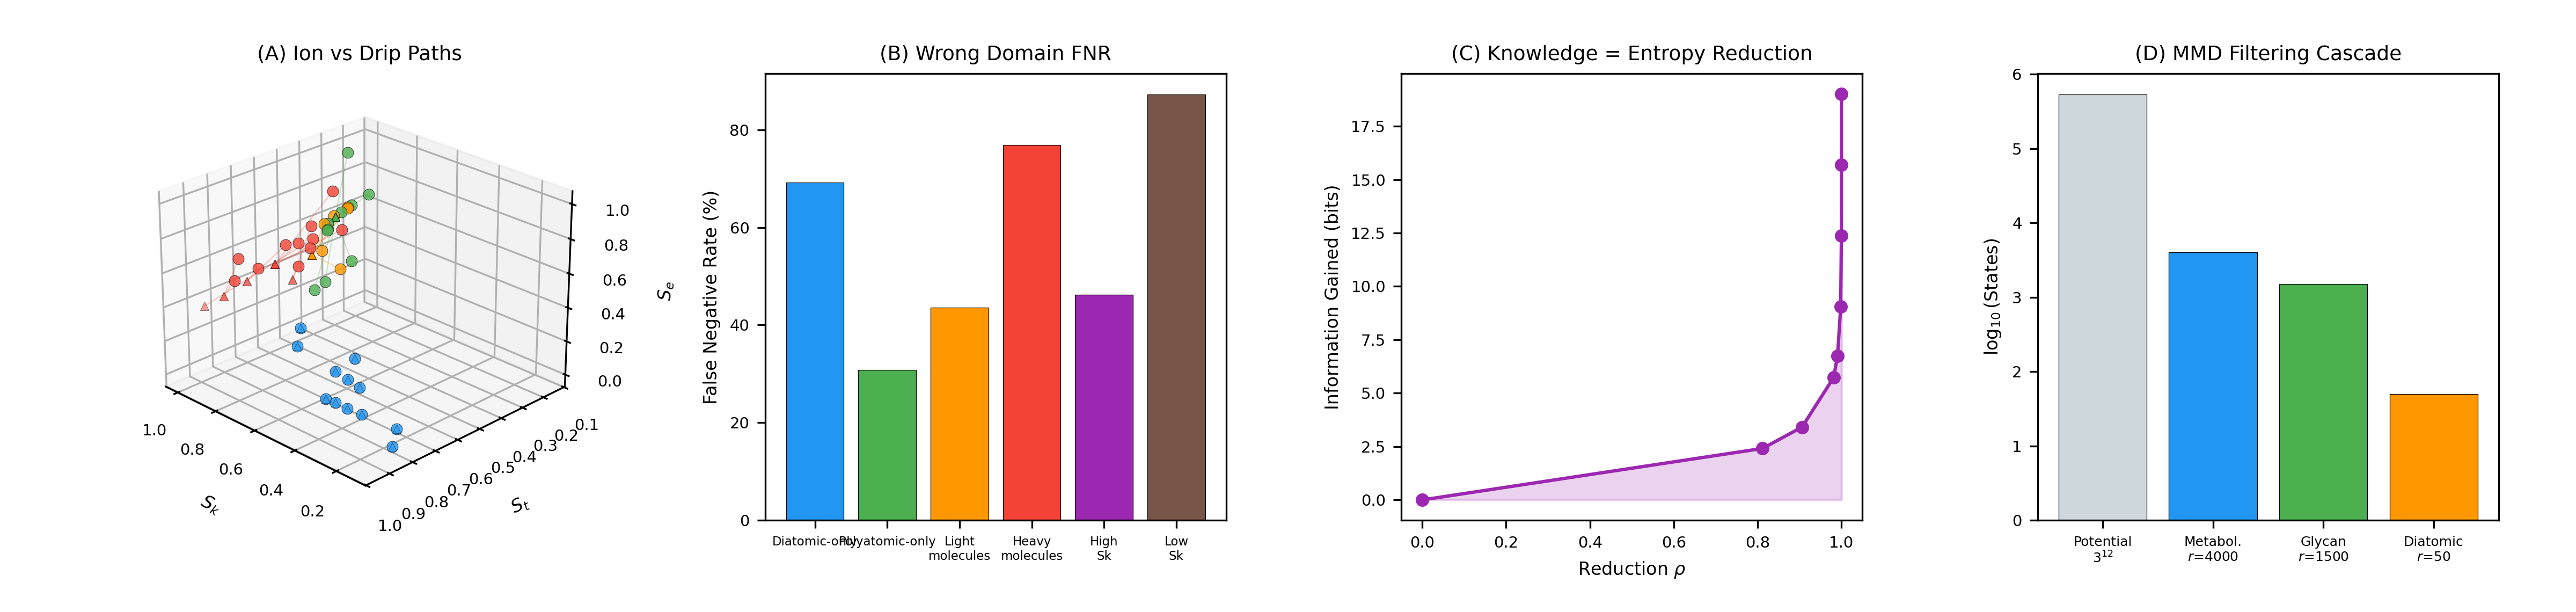
\includegraphics[width=\textwidth]{figures/panel_4_crossdomain_mmd.png}
    \caption{\textbf{Cross-Domain Validation and Molecular Maxwell Demon.}
    (\textbf{A})~Ion versus droplet paths in three-dimensional S-entropy space. Circles: ion-path coordinates ($S_k$, $S_t$, $S_e$); triangles: drip-path coordinates from Rayleigh surface modes. Connecting lines show the displacement between dual representations for each compound. Colour encodes molecular type. Short connecting lines indicate tight dual-path convergence; diatomics (blue, $S_e = 0$) show exact agreement on the $S_e$ coordinate, while polyatomics show small but systematic displacements reflecting the different physical basis of the two oscillatory representations.
    (\textbf{B})~Cross-domain false negative rate (FNR) when wrong domain constraints are applied. Restricting to ``diatomic only'' ($S_e < 0.01$) misses 69\% of compounds; ``heavy molecules'' ($m > 60$~Da) misses 77\%; ``low $S_k$'' ($S_k < 0.5$) misses 87\%. These high FNRs confirm domain specificity: constraints that exclude the target molecule produce identification failure, validating the Completeness Condition---accuracy loss is a property of incorrect constraints, not of the framework.
    (\textbf{C})~Knowledge as entropy reduction: information gained (bits) versus reduction ratio $\rho$. The curve rises steeply as $\rho \to 1$, reflecting the information-theoretic cost of narrowing the search. At $\rho = 0.99$ (99\% of phase space excluded), approximately 12 bits of domain knowledge have been applied. The relationship is monotonic and concave, consistent with Shannon's source coding theorem applied to the constrained region.
    (\textbf{D})~Molecular Maxwell Demon filtering cascade: $\log_{10}$ of accessible states at each filtering stage. The full potential space ($3^{12} = 531{,}441$ states) is progressively reduced by domain-specific MMD input filters: metabolomics ($r = 4{,}000$), glycomics ($r = 1{,}500$), diatomic gases ($r = 50$). Each stage represents a different MMD configuration applied to the same underlying phase space structure, demonstrating reconfigurability---the central property distinguishing Molecular Maxwell Demons from physical catalysts.}
    \label{fig:crossdomain_mmd}
\end{figure*}
